\chapter{Results and Discussion}
\label{sec:results}

\section{Effect of Pre-processing Images}
\todo[inline]{Compare tomo\_00058 denoising with and without cropping. Without cropping similar results to early stages of denoising cropped (i.e. poor and not converged). }

\begin{figure}[htbp]
  \centering
  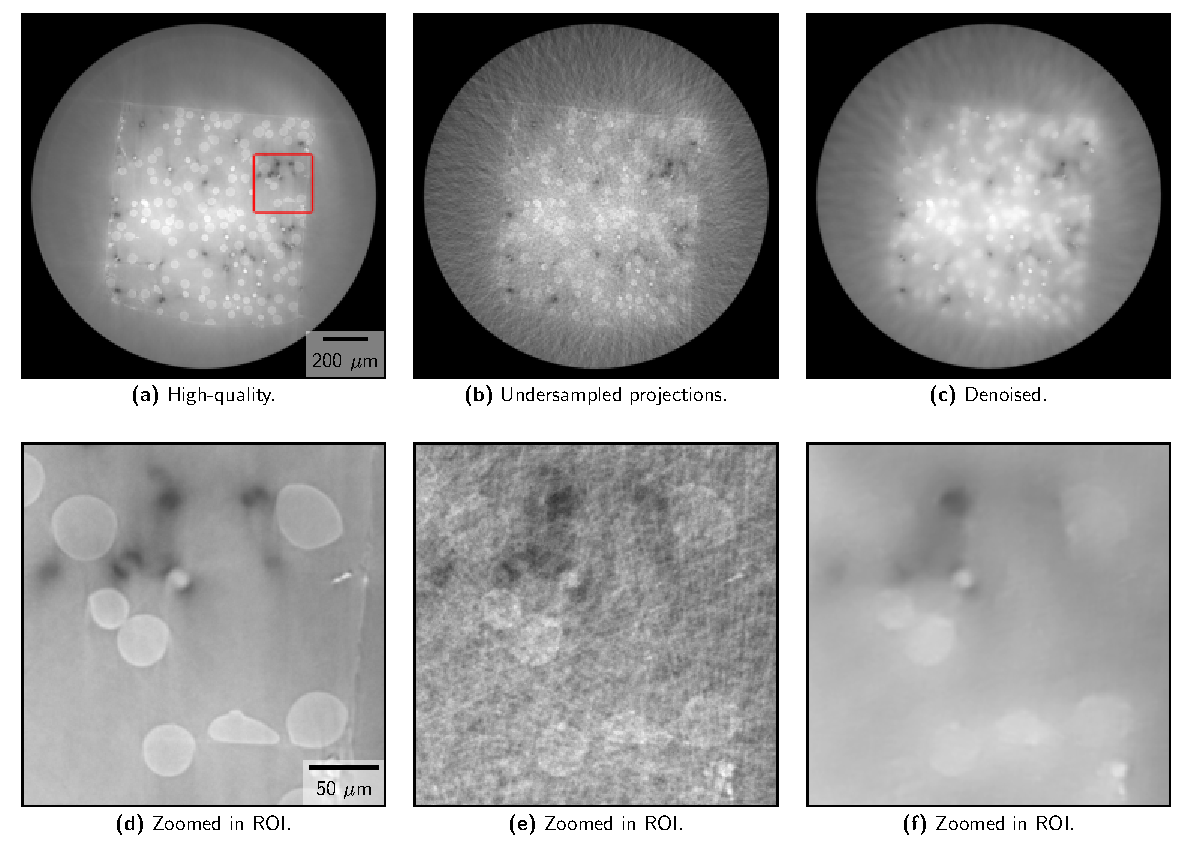
\includegraphics[width=.9\textwidth]{figures/uncroppeddenoising.pdf}
  \caption[Non-cropped image denoising]{Denoising of non-cropped dataset tomo\_00058. Images d), e), and f) are zoomed in \acrshort{roi}s of images a), b), and c) respectively. The \acrshort{roi} is marked in a). }
  \label{fig:uncroppeddenoising}
\end{figure}

\begin{figure}[htbp]
  \centering
  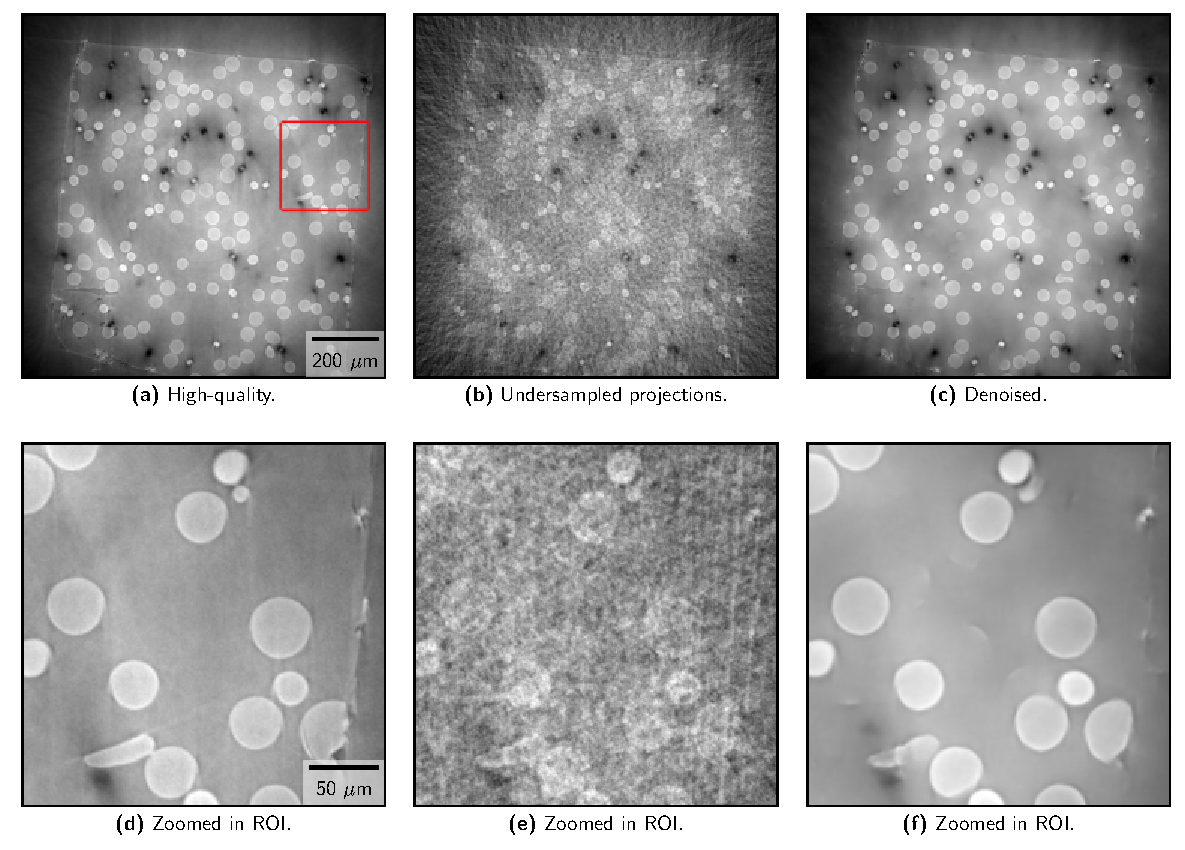
\includegraphics[width=.9\textwidth]{figures/croppeddenoising.pdf}
  \caption[Cropped image denoising]{Denoising of cropped dataset tomo\_00058. Images d), e), and f) are zoomed in \acrshort{roi}s of images a), b), and c) respectively. The \acrshort{roi} is marked in a). }
  \label{fig:croppeddenoising}
\end{figure}


\section{Hyperparameter and Loss Function Changes}
\todo[inline]{Show difference in tomo\_00058 denoising for different loss functions / weights (and hyperparameters?)}

\todo[inline]{Line plot of gt, ns, MSE denoising, Log-cosh denoising. Multiple lines around the images?}

\todo[inline]{SSIM and MSE evolution of arbitrary slice. }

\section{Different Amounts of Noise}
\todo[inline]{Different levels of noise / projection subsamplings (8,16,32,48). }
\todo[inline]{Plot of the images with zoomed in ROIs. }
\todo[inline]{Plot showing improvement in SSIM for different levels of noise. }
\todo[inline]{Line plot for different levels of noise? }




\section{Loss Function Evolution}
\todo[inline]{Plot how loss functions evolve through training of tomo\_00058 with good hyperparameters. }

\section{TomoGAN Compared to PICCS}
\todo[]{Change section name?}
\todo[inline]{Axial, sagittal, coronal plots for different depth parameters. }
\todo[inline]{Maybe make 3D model plot of this dataset. }
\todo[inline]{Line plot comparing GT, FDK?, PICCS, denoised. }
\todo[inline]{Histogram. Looks like peaks roughly align, sharper peaks. Looks like it is performing segmentation? Note: ordinate (y-axis) cropped to 20k. }
\todo[inline]{}

\begin{figure}
    \begin{subfigure}[t]{.45\textwidth}
      \centering
      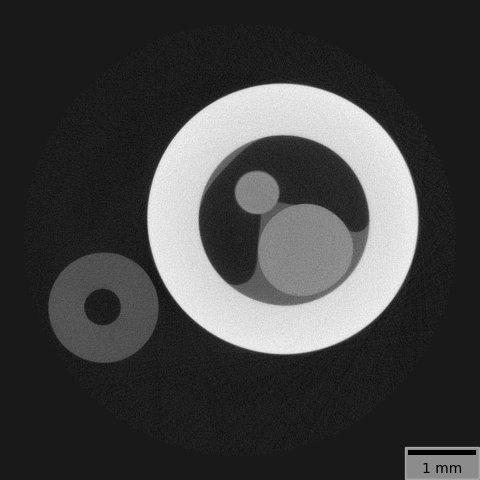
\includegraphics[width=\linewidth]{figures/kimrobertgt.png}
      \caption{High-quality. }
    \end{subfigure}
    \hfill
    \begin{subfigure}[t]{.45\textwidth}
      \centering
      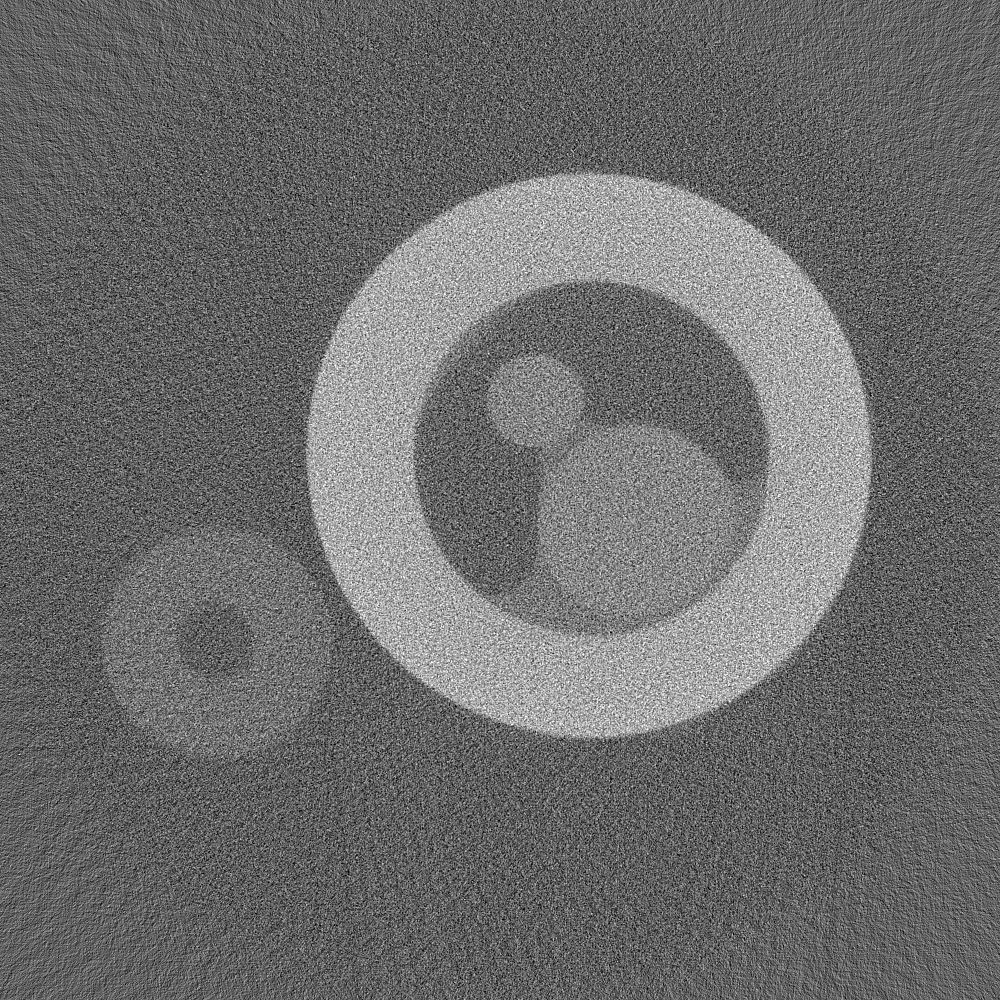
\includegraphics[width=\linewidth]{figures/kimrobertFDK.png}
      \caption{FDK.}
    \end{subfigure}
  
    \medskip
  
    \begin{subfigure}[t]{.45\textwidth}
      \centering
      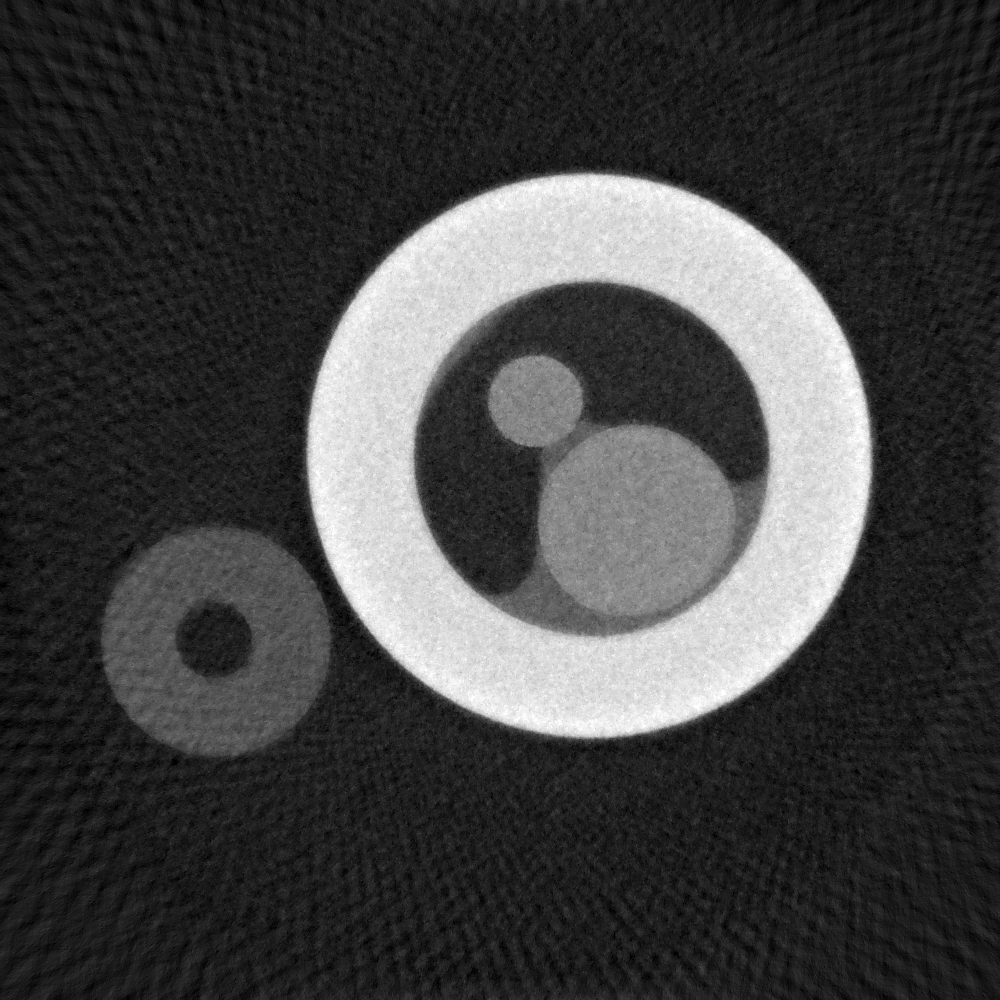
\includegraphics[width=\linewidth]{figures/kimrobertPICCS.png}
      \caption{PICCS. }
    \end{subfigure}
    \hfill
    \begin{subfigure}[t]{.45\textwidth}
      \centering
      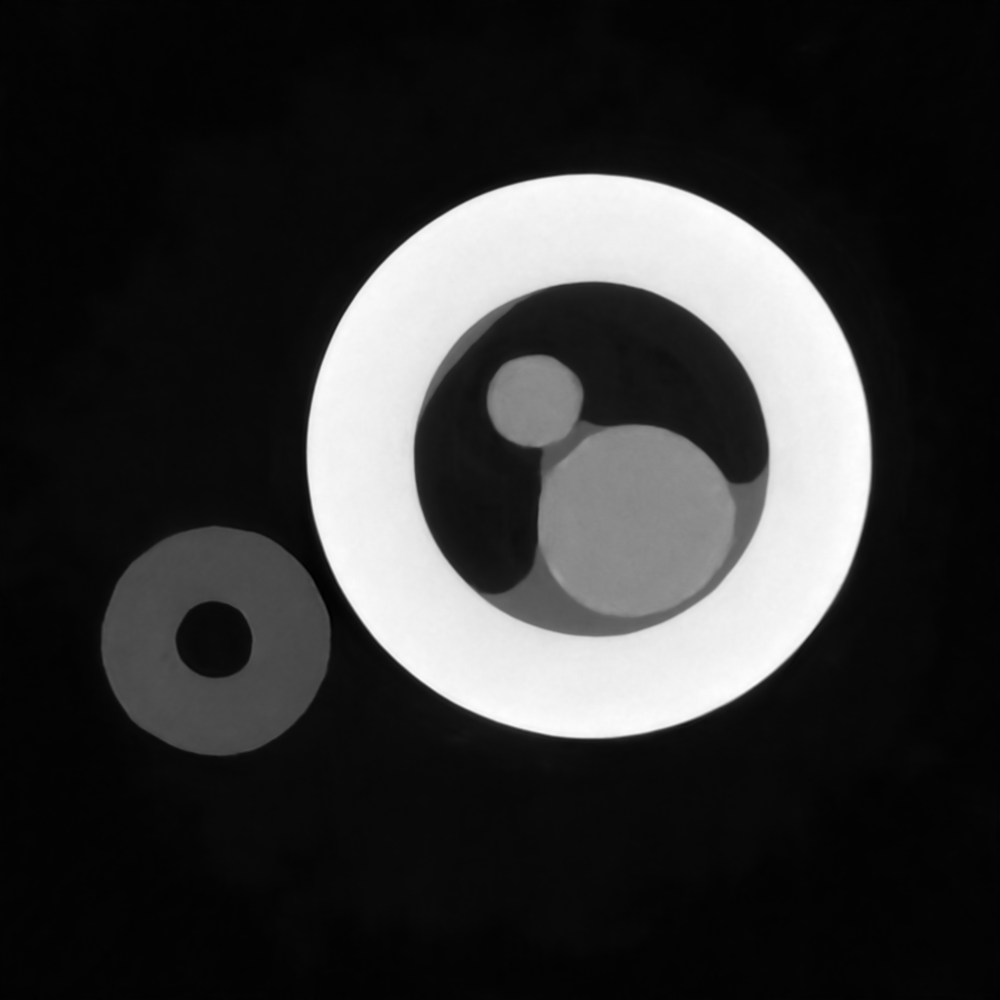
\includegraphics[width=\linewidth]{figures/kimrobertdepth1dn.png}
      \caption{FDK denoised. }
    \end{subfigure}
    \caption[Comparison of different reconstructions]{Comparison of different reconstructions. }
    \label{fig:kimrobertcomparison}
\end{figure}


\begin{figure}[htbp]
  \centering
  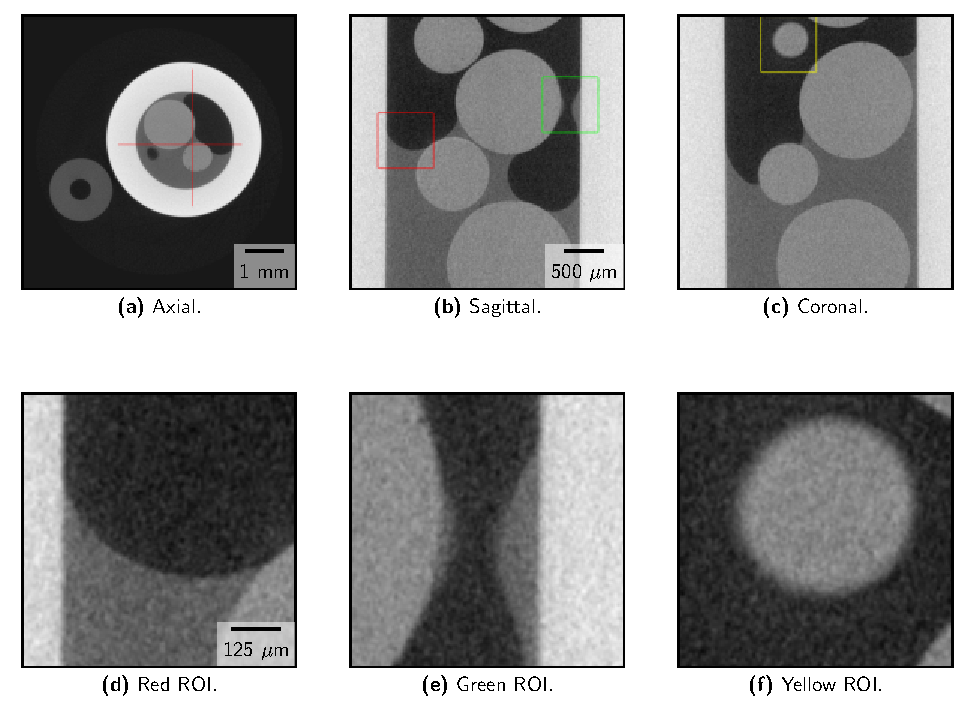
\includegraphics[width=.85\textwidth]{figures/kimroberthq-x475y620s250.pdf}
  \caption[High-quality]{View of the high-quality reconstruction. The red horizontal line in \textbf{(a)} corresponds to the sagittal view in \textbf{(b)}, and the red vertical line corresponds to the coronal view in \textbf{(c)}. Three \acrshort{roi}s have been marked in \textbf{(b)} and \textbf{(c)}, and can be seen in \textbf{(d)}-\textbf{(f)}. }
  \label{fig:sideplothq}
\end{figure}

\begin{figure}[htbp]
  \centering
  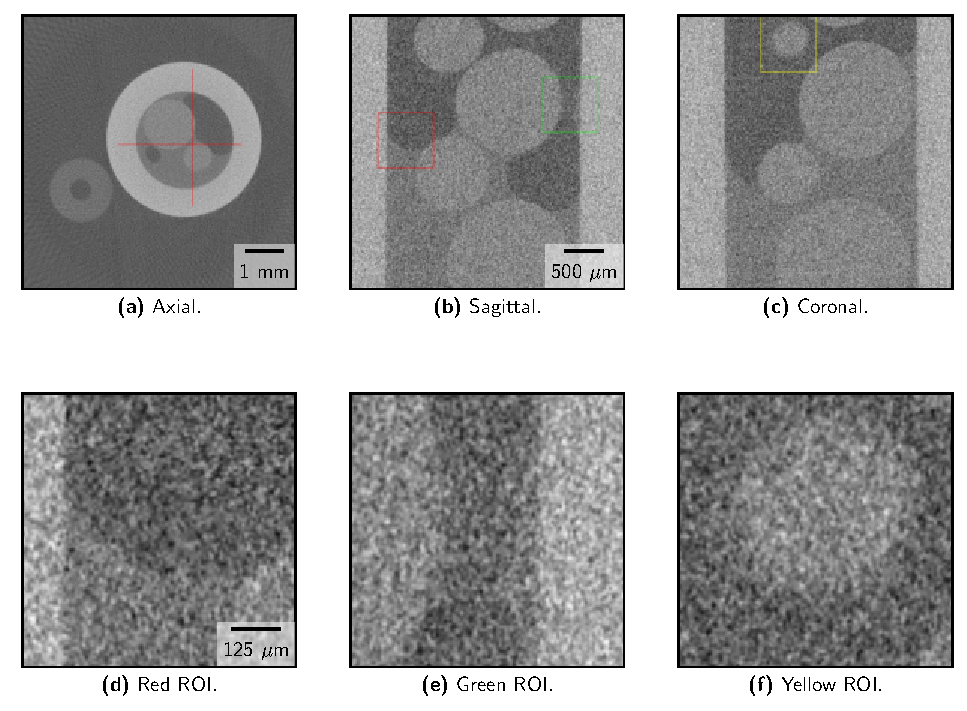
\includegraphics[width=.85\textwidth]{figures/kimrobertfdk-x475y620s250.pdf}
  \caption[FDK]{View of the FDK reconstruction. The red horizontal line in \textbf{(a)} corresponds to the sagittal view in \textbf{(b)}, and the red vertical line corresponds to the coronal view in \textbf{(c)}. Three \acrshort{roi}s have been marked in \textbf{(b)} and \textbf{(c)}, and can be seen in \textbf{(d)}-\textbf{(f)}. }
  \label{fig:sideplotfdk}
\end{figure}

\begin{figure}[htbp]
  \centering
  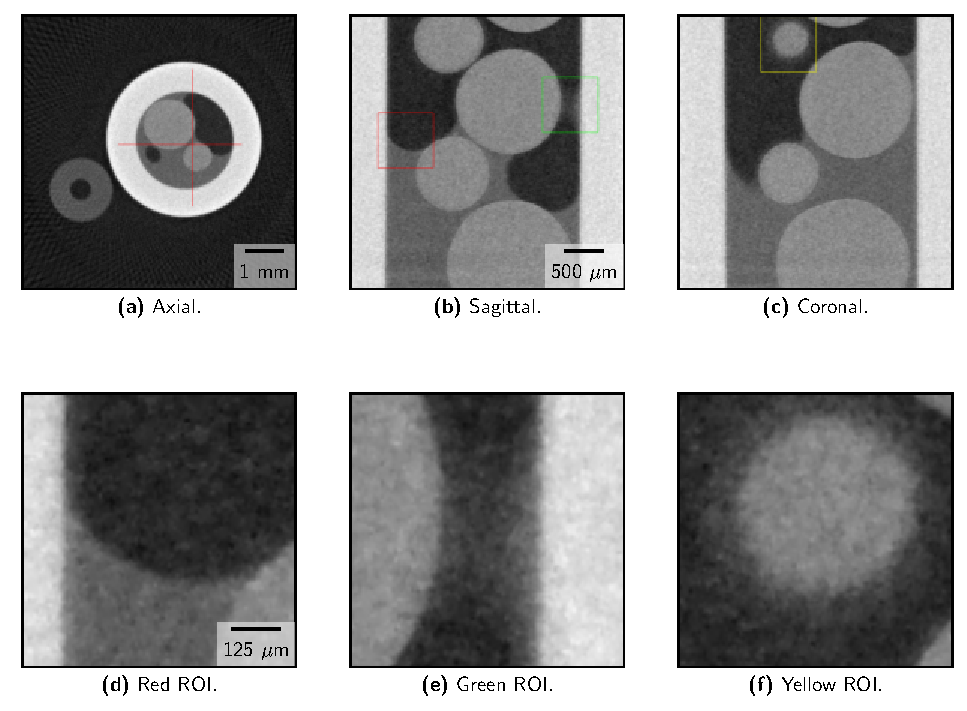
\includegraphics[width=.85\textwidth]{figures/kimrobertpiccs-x475y620s250.pdf}
  \caption[PICCS]{View of the PICCS reconstruction. The red horizontal line in \textbf{(a)} corresponds to the sagittal view in \textbf{(b)}, and the red vertical line corresponds to the coronal view in \textbf{(c)}. Three \acrshort{roi}s have been marked in \textbf{(b)} and \textbf{(c)}, and can be seen in \textbf{(d)}-\textbf{(f)}. }
  \label{fig:sideplotpiccs}
\end{figure}

\begin{figure}[htbp]
  \centering
  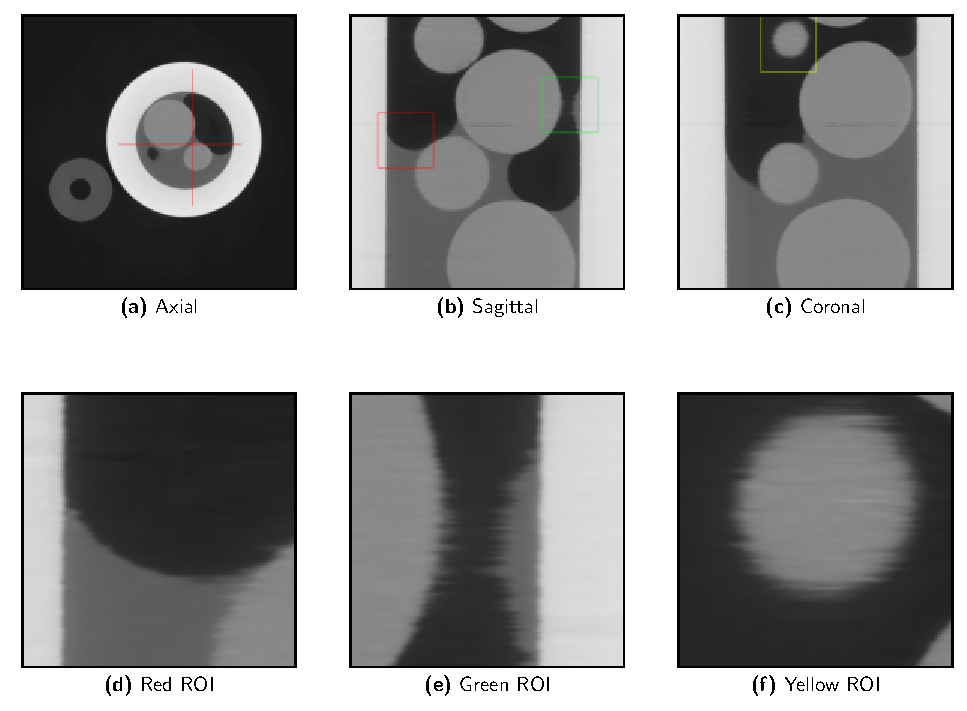
\includegraphics[width=.85\textwidth]{figures/kimrobertdepth1-x475y620s250.pdf}
  \caption[Depth=1]{View of the denoised FDK reconstruction with a depth of 1. The red horizontal line in \textbf{(a)} corresponds to the sagittal view in \textbf{(b)}, and the red vertical line corresponds to the coronal view in \textbf{(c)}. Three \acrshort{roi}s have been marked in \textbf{(b)} and \textbf{(c)}, and can be seen in \textbf{(d)}-\textbf{(f)}. }
  \label{fig:sideplotdepth1}
\end{figure}

\begin{figure}[htbp]
  \centering
  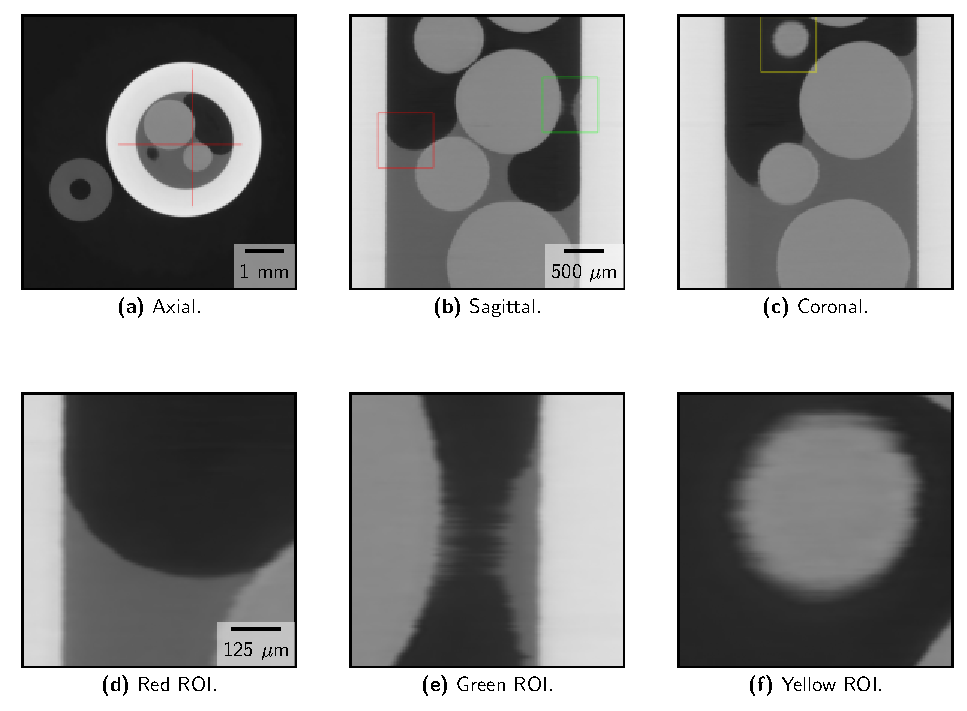
\includegraphics[width=.85\textwidth]{figures/kimrobertdepth3-x475y620s250.pdf}
  \caption[Depth=3]{View of the denoised FDK reconstruction with a depth of 3. The red horizontal line in \textbf{(a)} corresponds to the sagittal view in \textbf{(b)}, and the red vertical line corresponds to the coronal view in \textbf{(c)}. Three \acrshort{roi}s have been marked in \textbf{(b)} and \textbf{(c)}, and can be seen in \textbf{(d)}-\textbf{(f)}. }
  \label{fig:sideplotdepth3}
\end{figure}

\begin{figure}[htbp]
  \centering
  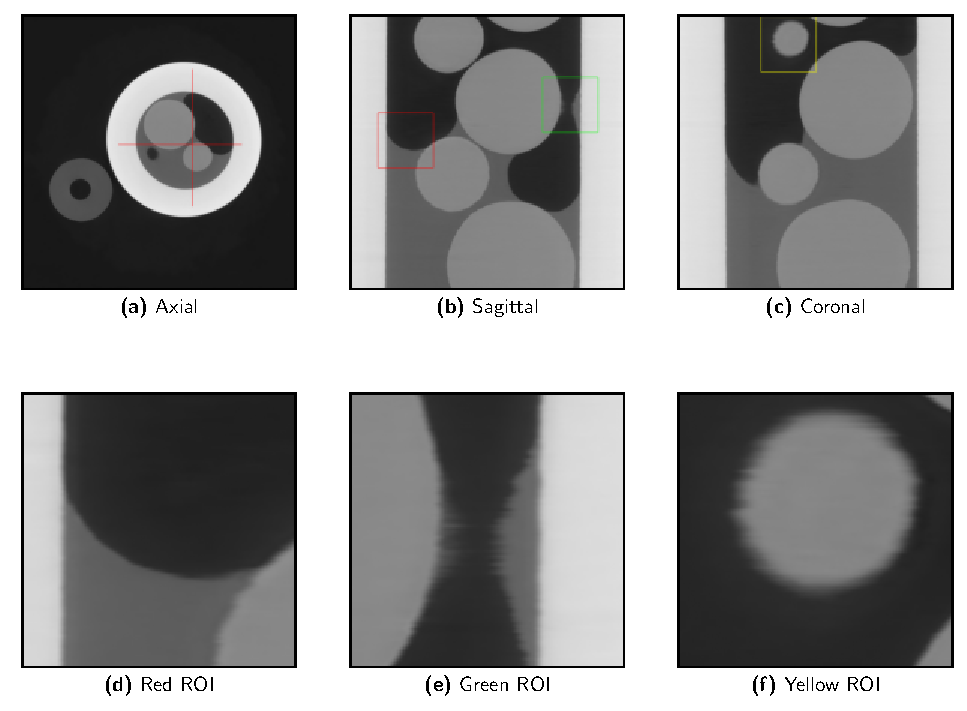
\includegraphics[width=.85\textwidth]{figures/kimrobertdepth5-x475y620s250.pdf}
  \caption[Depth=5]{View of the denoised FDK reconstruction with a depth of 5. The red horizontal line in \textbf{(a)} corresponds to the sagittal view in \textbf{(b)}, and the red vertical line corresponds to the coronal view in \textbf{(c)}. Three \acrshort{roi}s have been marked in \textbf{(b)} and \textbf{(c)}, and can be seen in \textbf{(d)}-\textbf{(f)}. }
  \label{fig:sideplotdepth5}
\end{figure}

\begin{figure}[htbp]
  \centering
  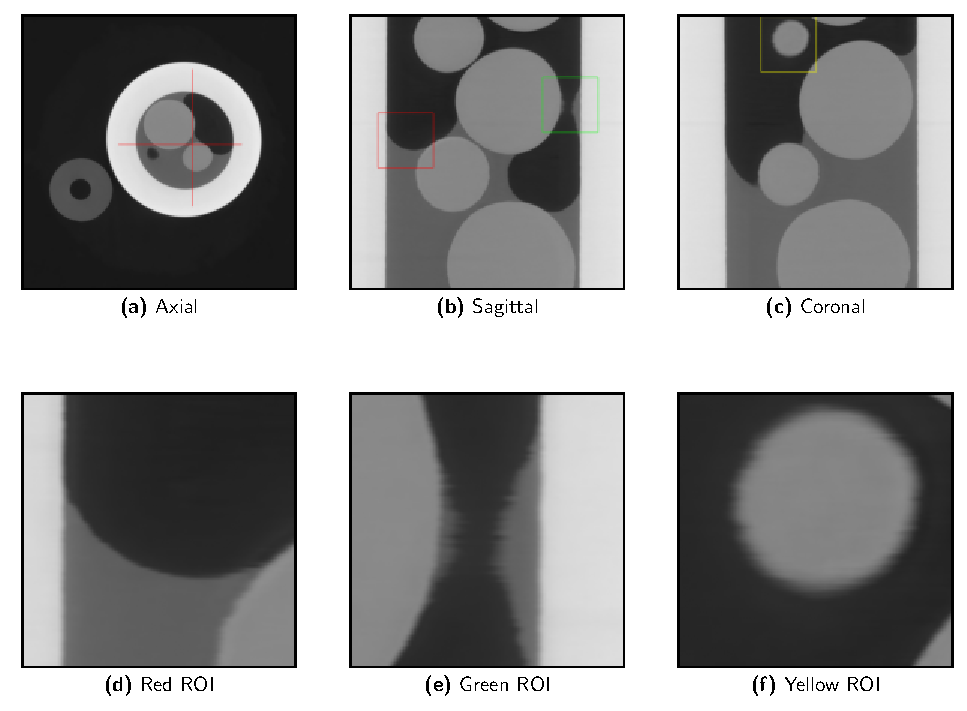
\includegraphics[width=.85\textwidth]{figures/kimrobertdepth7-x475y620s250.pdf}
  \caption[Depth=7]{View of the denoised FDK reconstruction with a depth of 7. The red horizontal line in \textbf{(a)} corresponds to the sagittal view in \textbf{(b)}, and the red vertical line corresponds to the coronal view in \textbf{(c)}. Three \acrshort{roi}s have been marked in \textbf{(b)} and \textbf{(c)}, and can be seen in \textbf{(d)}-\textbf{(f)}. }
  \label{fig:sideplotdepth7}
\end{figure}

\begin{figure}[htbp]
  \centering
  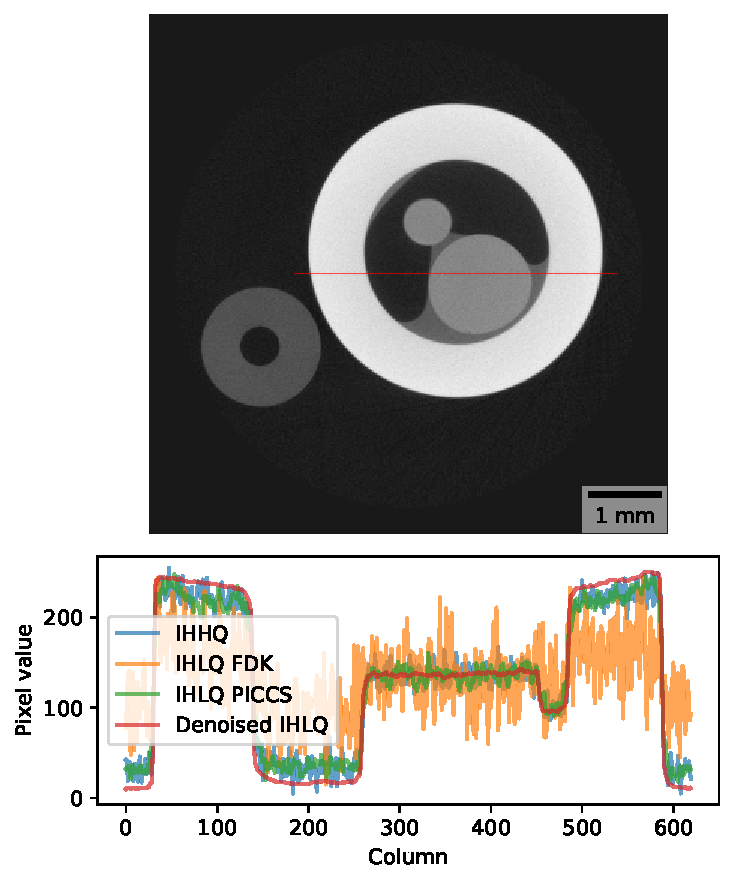
\includegraphics[width=.85\textwidth]{figures/kimrobertline.pdf}
  \caption[Line plot]{The plot shows pixel values for 620 pixels on a horizontal line, as shown by the red line on the high-quality image above. The denoised values are from denoising using a depth of 1. }
  \label{fig:line}
\end{figure}

\begin{figure}[htbp]
  \centering
  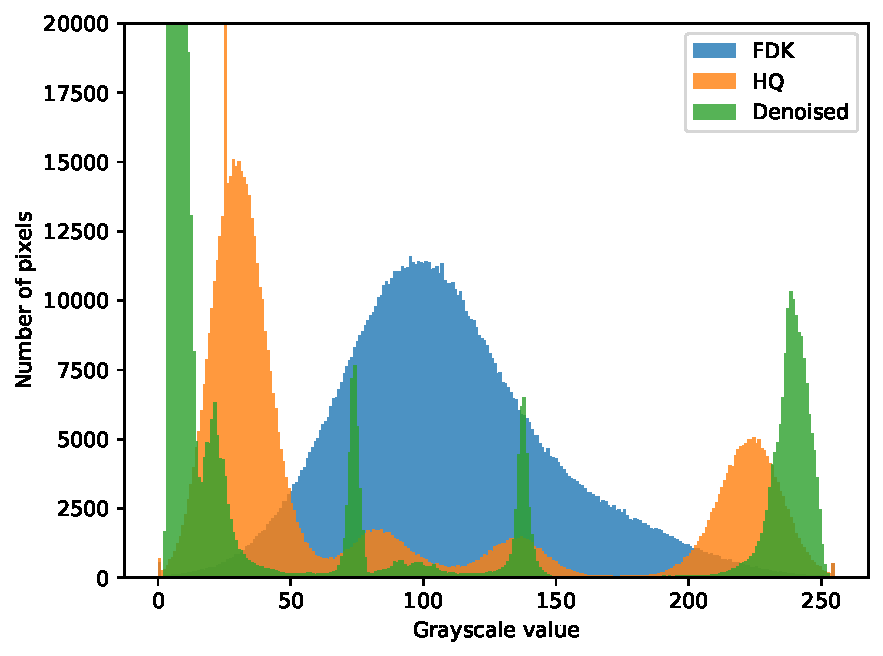
\includegraphics[width=.85\textwidth]{figures/kimroberthist.pdf}
  \caption[Histogram]{A histogram showing how the histogram of different reconstructions, including a denoised reconstruction, looks. Note that the ordinate has been cropped to a max value of $20000$. }
  \label{fig:hist}
\end{figure}

\section{Attempted Shale Denoising}
\todo[inline]{Include this?}
\todo[inline]{Shows limitations of method: requires a high-quality similar dataset (i.e. some ground truth) to work properly. Any given trained network doesn't work for all other dataset. }

Plot types: 
\begin{itemize}
    \item \acrshort{ssim} and \acrshort{mse} changes during training.
    \item Loss function evolution.
    \item Line plot of gt, ns, and different loss functions?
    \item Histograms of gt, ns, denoised
    \item Zoomed in region of interest.
    \item Axial, sagittal, and coronal plots of (at least Kim Robert's dataset) different depth parameters.
    \item Compare denoising of different subsamplings (8, 16, 32, 48)
    \item Activation plot of network layers.
\end{itemize}